\chapter{方法与系统实现}

\section{总体架构}

系统总体采用“文档解析-Embedding 与 Fusion-向量检索-Reranker 重排-路由决策-多模态生成-PDF 高亮溯源”的流水线。用户上传 PDF 或图片后，后端首先解析页面文本、页面图、表格、图像和局部区域；随后按 text、table、figure、code 等类型构建结构化 chunk，并通过统一文本-图像 embedding 接口建立索引。查询阶段，系统先通过 auto 路由或手动模式选择 Text-RAG、MM-RAG 或 ChartQA 专用路径，再召回与重排证据，最后由生成模型输出答案和引用信息。前端负责展示知识库 chunk、连续 PDF 预览和答案高亮区域。

\begin{figure}[htbp]
  \centering
  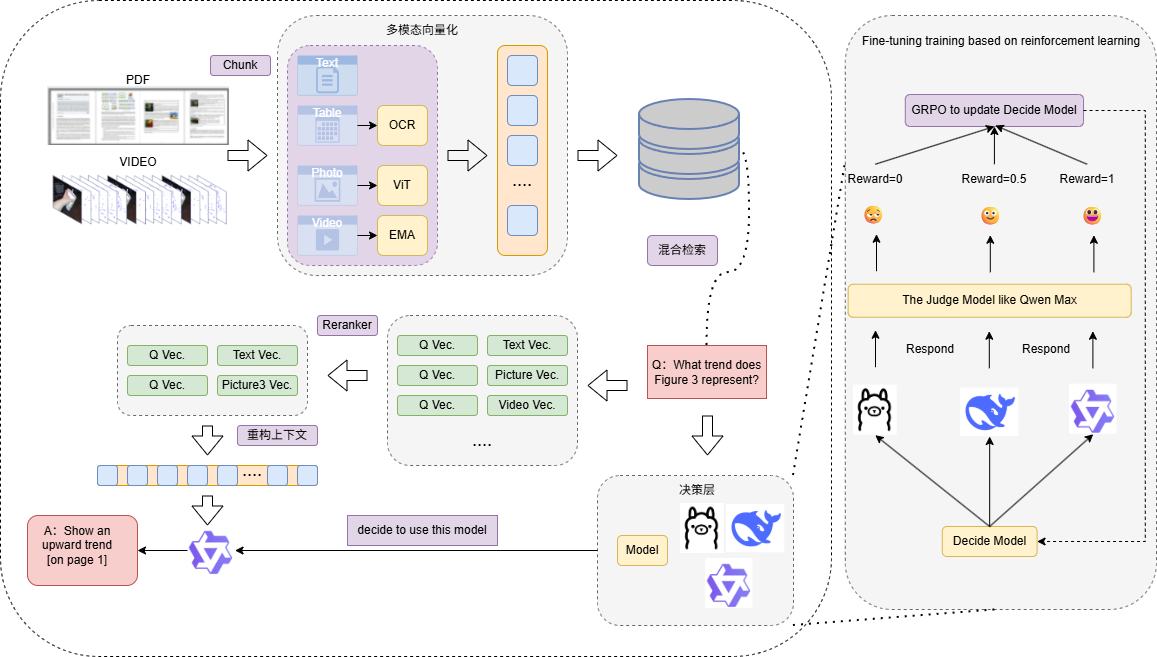
\includegraphics[width=0.95\textwidth]{image/frame.png}
  \caption{系统总体架构图}
  \label{fig:system_architecture}
\end{figure}

图 \ref{fig:system_architecture} 展示了开题阶段设计的总体架构。期末实现保留了其中“多模态知识库+检索重排+路由生成+溯源展示”的主线，但做了工程化调整：GRPO 学习式路由没有完整训练，而是实现为 GRPO-style auto router、候选 VLM 打分和策略更新钩子；多模态向量化没有训练大型跨模态模型，而是实现统一文本-图像 embedding 接口、轻量图像特征和可选 Native ViT 图像编码器；前端从单页/单 chunk 展示调整为连续 PDF 预览和区域高亮。

\section{文档解析实现}

文档解析对应第二章中的“文档解析与 OCR”组件，主要由 ingest.py 模块实现。对于 PDF 文件，系统使用 PyMuPDF 抽取每页文本，并将每页渲染为 PNG 页面图；对于图片文件，系统直接将其视为单页文档。解析后，每一页都包含页码、页面文本、页面图路径、页面宽度和页面高度。

在此基础上，系统将页面内容进一步切分为 chunk。文本 chunk 只保留普通段落文本；代码段会被识别为 code chunk；表格区域会被 PyMuPDF 表格检测抽出并转换为 Markdown table，作为 table chunk 入库；页面图片、图表和公式区域会被裁剪为 figure 或 formula chunk。已识别的表格、图片和公式区域会从普通页面文本中排除，避免同一内容既污染 text chunk，又作为结构化 chunk 重复出现。这里的 bbox、image path、page width 和 page height 都使用普通字段保存，前端可以据此把证据位置映射回 PDF 页面。

文档解析模块解决的是“知识从哪里来”的问题。它不仅为后续 embedding 提供文本，也为 VLM 提供页面图和局部视觉区域，是 Text-RAG 与 MM-RAG 共用的基础。

\section{Embedding 与 Fusion 实现}

Embedding 对应语义向量化功能，主要由 model\_stack.py、real\_models.py 和 multimodal\_embeddings.py 管理。真实模型模式下，系统使用 BGE-M3 生成文本 chunk 的向量表示，并使用 FAISS 建立向量索引。图像侧默认使用轻量图像特征编码器，将颜色、比例、视觉 token 等信息映射为向量；如果配置了图像 embedding 模型，也可以使用 Native ViT 图像编码器。用户问题到来后，问题同样被编码为向量，用于和知识库 chunk 进行相似度匹配。

Fusion 的实现分为两层。第一层是向量层融合：统一文本-图像 embedder 会把文本向量和图像向量按权重融合，并在 metadata 中记录 embedding modalities 与 embedding space。第二层是 evidence 层融合：一个 evidence 可以同时包含文本内容、页码、页面图路径、bbox、OCR 文本、局部 crop、表格 Markdown 和来源类型。这样做的好处是：检索阶段可以利用统一向量空间快速召回，生成阶段可以把对应页面图、局部 crop 或表格结构交给 VLM 进一步理解。

因此，本项目中的 Fusion 更偏向工程融合：文本负责召回，视觉区域负责补充理解，坐标信息负责溯源展示。它实现了开题报告中“文本、表格和图像信息共同进入多模态 RAG 流程”的目标。

\section{向量检索与 Reranker 实现}

向量检索和 Reranker 对应第二章中的知识问答核心组件，主要在 pipeline.py 中组织。系统首先用向量索引召回 Top-K 候选 evidence，再使用 BGE-reranker-v2-m3 对问题和候选证据进行二次打分。重排后，系统只保留最相关的证据输入生成模型，减少无关 chunk 对回答的干扰。

在 Text-RAG 路径中，检索和重排直接决定最终上下文；在 MM-RAG 路径中，检索和重排还承担“定位视觉证据”的作用。例如，当问题涉及某个图表、品牌或日程表时，文本检索先帮助系统找到相关页面或相关 OCR 片段，再由视觉区域生成模块裁剪局部 crop。这样，Reranker 不只是提高文本答案质量，也间接提高了 VLM 看到正确区域的概率。

最终 prompt 中，证据会被组织成带编号的片段，如 [E1]、[E2]。模型只需要引用证据编号，后端再把编号映射为具体页码、chunk 和 bbox，避免模型自己编造来源。

\section{路由决策实现}

路由决策对应开题报告中的 GRPO 自动路由模块。原计划中，系统希望通过 GRPO 训练轻量化路由模型，让它根据问题类型选择不同 VLM 或不同处理路径。期末阶段，考虑到训练样本、评分模型和时间限制，项目没有完整训练 Qwen-0.5B 路由器，而是实现了 GRPO-style auto router，作为自动路由的可运行版本。

当前路由逻辑主要分为三类。第一，普通定义、摘要、章节内容查找等问题进入 Text-RAG，直接使用文本 chunk 检索和生成。第二，涉及图片、表格、图表、logo、广告、商品标签或页面区域的问题进入 MM-RAG，系统会优先准备页面图或局部 crop。第三，ChartQA 样本进入图表专用 route，固定生成 chart region，并在 prompt 中加入 compare、difference、max、min、average 等图表任务提示。当前前端默认模型入口为 auto，对应后端自动路由流程；后端会返回 route、retrieval modes、selected model 和 policy trace，便于后续检查和训练。

这一路由实现虽然没有经过真实强化学习训练，但已经完成了“根据问题类型选择合适处理路径”的功能，并保留 grouped rewards 策略更新钩子。后续如果继续扩展 GRPO，只需要把当前 auto 路由产生的路径选择、答案结果和人工/自动评分保存为训练数据，就可以训练更轻量的 route policy。

\section{VLM 与局部视觉区域实现}

VLM 多模态生成主要由真实模型 backend 调用 Qwen3-VL-8B-Instruct 完成。系统不会把所有页面无差别送入 VLM，而是先通过检索、OCR bbox 和问题关键词缩小候选范围，再裁剪局部高清 crop。这样可以降低视觉 token 成本，也能减少页面其他内容对模型的干扰。

局部区域生成主要由 vision\_regions.py 完成。对于 DocVQA 中的数字、年份、广告品牌、商品标签和日程表问题，系统根据 OCR bbox 和关键词生成候选区域；对于 ChartQA，系统优先裁剪图表主体区域；对于 PDF 中检测到的表格和图片区域，系统会保留裁剪图、结构化 metadata 和可用于前端展示的 preview。实际评测中，局部 crop 对 ChartQA 和视觉实体问题提升明显，说明 VLM 的作用不是简单“多看一张图”，而是需要配合检索和区域选择，把视觉模型的注意力集中在高价值证据上。

\section{FastAPI 服务层实现}

FastAPI 服务层主要由 api.py 实现，负责把后端 pipeline 封装为前端可调用的接口。它维护文件状态、解析任务状态、chunk 列表、页面图和问答结果，使前端可以轮询解析进度并展示知识库内容。

\begin{table}[htbp]
  \centering
  \caption{FastAPI 主要接口}
  \label{tab:api}
  \begin{tabular}{p{0.32\textwidth}p{0.58\textwidth}}
    \toprule
    接口 & 功能 \\
    \midrule
    POST /files & 上传一个或多个 PDF/图片文件。\\
    POST /files/id/parse & 启动解析、渲染、chunk 构建与索引。\\
    GET /jobs/id & 查询解析进度和错误信息。\\
    GET /files/id/chunks & 返回知识库 chunk 列表。\\
    GET /pages/image & 返回 PDF 页面渲染图。\\
    POST /query & 执行检索问答，返回答案、引用和证据。\\
    DELETE /files/id & 删除上传文件、处理结果和预览缓存。\\
    \bottomrule
  \end{tabular}
\end{table}

服务层支持 uploaded、queued、parsing、ready 和 failed 等状态。对于真实模型 API 欠费、权限不足或解析失败等情况，后端会返回结构化错误，前端可以显示友好提示，而不是直接暴露原始供应商报错。

\section{前端 PDF 预览与高亮实现}

前端主界面由 App.tsx 实现，使用 React、Vite、TailwindCSS 和 Framer Motion。最终界面采用左右双栏：左侧是文件、知识库 chunk 和问答结果，右侧是连续 PDF 预览。用户选中某个 chunk 或答案引用后，右侧 PDF viewer 自动滚动到对应页，并根据 bbox 绘制高亮框。

这个设计对应第二章中的“PDF 高亮与可解释溯源”。与只显示某个 chunk 文本不同，连续 PDF 预览可以让用户上下翻页检查文档上下文；高亮框则把 evidence 从抽象的 chunk 还原到原始页面区域。这样用户能判断答案是否真的来自文档，而不是模型凭空生成。

\section{代码结构}

项目代码按前后端和评测脚本组织，主要文件如表 \ref{tab:repo_structure} 所示。这里使用普通正文样式列出路径，避免正文中出现突兀的等宽字体。

\begin{table}[htbp]
  \centering
  \caption{项目主要代码结构}
  \label{tab:repo_structure}
  \begin{tabular}{p{0.38\textwidth}p{0.52\textwidth}}
    \toprule
    路径 & 功能 \\
    \midrule
    frontend/ & React + Vite 前端。\\
    src/mllmproject/api.py & FastAPI 服务层。\\
    src/mllmproject/ingest.py & 文档解析、页面渲染与结构化区域抽取。\\
    src/mllmproject/pipeline.py & RAG 主流程。\\
    src/mllmproject/ \newline model\_stack.py & 模型栈、统一 embedding 与 backend 切换。\\
    src/mllmproject/ \newline multimodal\_embeddings.py & 文本-图像统一向量空间。\\
    src/mllmproject/ \newline grpo\_router.py & GRPO-style auto router 与策略更新钩子。\\
    src/mllmproject/ \newline table\_markdown.py & 表格 Markdown 结构化。\\
    src/mllmproject/ \newline real\_models.py & BGE 与 Qwen3-VL 适配器。\\
    src/mllmproject/ \newline vision\_regions.py & OCR bbox 与局部 crop。\\
    src/mllmproject/evaluation.py & 评测流程。\\
    scripts/ & 批量评测与 demo 脚本。\\
    data/eval/ & 评测样本与结果。\\
    Report/ & 开题报告、期末报告和参考文献。\\
    \bottomrule
  \end{tabular}
\end{table}

仓库 README 中提供了环境配置、命令行评测、React + FastAPI 联调和 Gradio demo 的运行方式，满足课程对代码仓库和运行说明的要求。
